%% -*- TeX-master: t -*-

%% \documentclass[draft]{acm_proc_article-sp}
\documentclass[draft]{sig-alternate}


%%%%%%%%%%%%%%%%%%%%%%%%%%%%%%%%%%%%%%%%%%%%%%%%%%%%%%%%%%%%%%%%%%%%%%%%
%%
%% standard texmf packages
%%

\usepackage{amsmath}
\usepackage{booktabs}
\usepackage{graphicx}
\usepackage{ifthen}
\usepackage{nicefrac}
\usepackage{fancyvrb}
\usepackage[scrtime]{prelim2e}
\usepackage[TABTOPCAP]{subfigure}
\usepackage{url}
\usepackage{xspace}

\usepackage{mathptmx}
\usepackage{times}
\DeclareMathAlphabet{\mathcal}{OMS}{cmsy}{m}{n}

\usepackage[
bookmarks,
breaklinks,
draft=false,
pdftitle={Scalable Statistical Debugging},
pdfauthor={Ben Liblit, Mayur Naik, Alice X. Zheng, Alex Aiken, and Michael I.  Jordan},
pdfsubject={D.2.4 [Software Engineering]: Software/Program Verification -- statistical methods; D.2.5 [Software Engineering]: Testing and Debugging -- debugging aids, distributed debugging, monitors, tracing; I.5.2 [Pattern Recognition]: Design Methodology -- feature evaluation and selection},
pdfkeywords={bug isolation, random sampling, invariants, feature selection, statistical debugging},
pdfpagemode=UseOutlines
]{hyperref}

\ifthenelse{\isundefined{\pdfoutput}}{}{\usepackage{thumbpdf}}

%% \VerbatimFootnotes


%%%%%%%%%%%%%%%%%%%%%%%%%%%%%%%%%%%%%%%%%%%%%%%%%%%%%%%%%%%%%%%%%%%%%%%%
%%
%% unique to this paper
%%

\usepackage{views/bug-o-meter}
\usepackage{views/view}

\renewcommand{\sectionautorefname}[0]{Section}
\renewcommand{\subsectionautorefname}[0]{\sectionautorefname}
\newcommand{\subtableautorefname}[0]{\tableautorefname}

\newtheorem{theorem}{Theorem}[section]
\newtheorem{lemma}[theorem]{Lemma}

\newcommand{\moss}{\textsc{Moss}\xspace}
\newcommand{\rhythmbox}{\textsc{Rhythmbox}\xspace}
\newcommand{\exif}{\textsc{exif}\xspace}
\newcommand{\bc}{\textsc{bc}\xspace}
\newcommand{\ccrypt}{\textsc{ccrypt}\xspace}
\newcommand{\termdef}[1]{\emph{#1}}
\newcommand{\prob}{\ensuremath{\textit{Pr}}}
\newcommand{\fail}{\ensuremath{\textit{Crash}}}
\newcommand{\crash}{\ensuremath{\textit{Failure}}}
\newcommand{\context}{\ensuremath{\textit{Context}}}
\newcommand{\increase}{\ensuremath{\textit{Increase}}}
\newcommand{\importance}{\ensuremath{\textit{Importance}}}
\newcommand{\numfail}{\ensuremath{\textit{NumF}}}
\renewcommand{\H}{{\mathcal{H}}}
\newcommand{\report}[1]{\ensuremath{R[#1]}}

\newcommand{\issue}[2][]{}


%%%%%%%%%%%%%%%%%%%%%%%%%%%%%%%%%%%%%%%%%%%%%%%%%%%%%%%%%%%%%%%%%%%%%%%%
%%
%% front matter
%%



\title{Scalable Statistical Debugging
  %%
  \renewcommand{\footnotemark}[0]{}
  %%
  \thanks{This research was supported in part by NSF Grant Nos.\
    EIA-9802069, CCR-0085949, ACI-9619020, and IIS-9988642; NASA Grant
    No.\ NAG2-1210; DOE Prime Contract No.\ W-7405-ENG-48 through
    Memorandum Agreement No.\ B504962 with LLNL; and DARPA ARO-MURI
    ACCLIMATE DAAD-19-02-1-0383.  The information presented here does
    not necessarily reflect the position or the policy of the
    Government and no official endorsement should be inferred.}}

\makeatletter
\newcommand*{\eecsMark}[0]{\@fnsymbol{1}}
\newcommand*{\statMark}[0]{\@fnsymbol{2}}
\newcommand*{\stanMark}[0]{\@fnsymbol{3}}
\makeatother
\newcommand*{\eecs}[0]{\textsuperscript{\eecsMark}}
\newcommand*{\stat}[0]{\textsuperscript{\statMark}}
\newcommand*{\both}[0]{\textsuperscript{\eecsMark, \statMark}}
\newcommand*{\stan}[0]{\textsuperscript{\stanMark}}

\newcommand{\moreauthors}[0]{\end{tabular}\\\begin{tabular}[t]{c}}

\author{%
  Ben Liblit \eecs
  \and Mayur Naik \stan
  \and Alice X.\ Zheng \eecs
  \and Alex Aiken \stan
  \and Michael I.\ Jordan \both
  \moreauthors
  \eecs Department of Electrical \\
  Engineering and Computer Science \\
  \stat Department of Statistics \\
  University of California, Berkeley \\
  Berkeley, CA 94720-1776
  \and
  \stan Computer Science Department \\
  Stanford University \\
  Stanford CA 94305-9025
}

\bibliographystyle{abbrv}


%%%%%%%%%%%%%%%%%%%%%%%%%%%%%%%%%%%%%%%%%%%%%%%%%%%%%%%%%%%%%%%%%%%%%%%%
%%
%%  document body
%%


\begin{document}

\issue[Mike]{I think that Section 5.1 would be better placed at the
end of Section 4.}

\maketitle

\begin{abstract}
  We present a statistical debugging algorithm that is
  robust in the face of multiple undiagnosed bugs.  The algorithm
  identifies program behaviors that significantly increase the
  likelihood of failure; these predictors reveal both the
  circumstances under which bugs occur as well as the frequencies of
  failure modes, making it easier to prioritize debugging efforts.
  Our algorithm is validated using several case studies, including finding
  previously unknown and significant crashing bugs in widely used systems.
  We compare our technique with an earlier algorithm and find it much more accurate 
  and scalable.
\end{abstract}


%\category{D.2.4}{Software Engineering}{Software/Program
%  Verification}[statistical methods]
%%
%\category{D.2.5}{Software Engineering}{Testing and
%  Debugging}[debugging aids, distributed debugging, monitors, tracing]
%%
%\category{I.5.2}{Pattern Recognition}{Design Methodology}[feature
%  evaluation and selection]

%\terms{Experimentation, Reliability}

%\keywords{bug isolation, random sampling, invariants, feature
%  selection, statistical debugging}


\section{Introduction}
\label{sec:introduction}

\issue[Alice]{Too much notation in introduction?}

This paper is about \termdef{statistical debugging}, a dynamic
analysis for identifying the causes of software failures (i.e., bugs).
Instrumented programs monitor their own behavior and send feedback
reports to a central collection server.  The instrumentation examines
program behavior during execution by sampling; complete information is
never available about any single run.  However, monitoring is also
lightweight and therefore practical to deploy to large user
communities, making it possible to gather information about many runs.
The collected data can then be analyzed for interesting trends across
all of the monitored executions.

In our approach, instrumentation consists of \termdef{predicates} tested
at particular program points; we defer discussing which predicates are
chosen for instrumentation to \autoref{sec:background}.  A given
program point may have many predicates that are sampled independently
during program execution when that program point is reached (i.e.,
each predicate associated with a program point may or may not be
tested each time the program point is reached).  A feedback report $R$
consists of one bit indicating whether a run of the program
succeeded or failed, as well as a bit vector with one bit for each
predicate $P$; if $P$ is observed to be true at least once during run
$R$ then $\report{P} = 1$, otherwise $\report{P} = 0$.
    
\issue{modified by Alice}

The usual definition of a bug refers to a programmatic element that 
unintentionally causes incorrect behavior.  We're going to abuse notation a
bit and overload its definition.  In this paper, a \termdef{bug} also refers to
a set of failing runs (feedback reports) ${\cal B}$
that share a cause of failure.  The meaning becomes clear in context.  The 
union of all bugs is exactly the
set of failing runs, but note that ${\cal B}_i \cap {\cal B}_j \neq
\emptyset$ in general; more than one bug can occur in some runs.

\issue[Mike]{"A bug is a set of failing runs".  Semantically one thinks 
of a bug as someone that characterizes a program, not a set of runs.
What about calling a set of a failing runs a "bug profile"?}

A predicate $P$ is a \termdef{bug predictor} (or simply a
\termdef{predictor}) of bug ${\cal B}$ if whenever $\report{P} = 1$
then it is statistically likely that $R \in {\cal B}$ (see
\autoref{sec:increase}).  \termdef{Statistical debugging} selects a
small subset ${\cal S}$ of the set of all instrumented predicates
${\cal P}$ such that ${\cal S}$ has predictors of all bugs.  We also
rank the predictors in ${\cal S}$ from the most to least important.
The set ${\cal S}$ and associated metrics (see
\autoref{sec:experiments}) are then available to engineers to help
speed the process of finding and fixing the most serious bugs.

In previous work, we focused on techniques
for lightweight instrumentation and sampling of program executions, but
we also studied two preliminary algorithms for statistical debugging and
presented experimental results on medium-size applications with a
single bug \cite{PLDI`03*141,NIPS2003_AP05}.  The most general
technique we studied is \termdef{regularized logistic regression}, a standard
statistical procedure that tries to select a set of predicates that
best predict the outcome of every run. As we worked to apply these
methods to much larger programs under realistic conditions, we
discovered a number of serious scalability problems:

\begin{itemize}

\item For large applications the set ${\cal P}$ numbers in the hundreds of
thousands of predicates, many of which are, or are very nearly,
logically redundant.  In our experience, this redundancy in ${\cal P}$
causes logistic regression to choose highly redundant lists of
predictors ${\cal S}$.  Redundancy is
already evident in prior work \cite{PLDI`03*141} but becomes much
worse for larger programs.
%%
\issue[Alice]{Logistic regression is not a global optimization
  technique.  The fact that predictors for less common bugs are ranked
  lower by logistic regression is a consequence of doing binary
  classification when we really should be doing multi-class
  classification.  But we can't do multi-class classification since we
  don't know the underlying bug labels. [text modified]}

\item A separate difficulty is the prevalence of predicates predicting
multiple bugs.  For example, for many Unix programs a bug is more
likely to be encountered when many command line flags are given,
because the more options that are given non-default settings the more
likely unusual code paths are to be exercised.  Thus, predicates
implying a long command line may rank near the top, even though such
predicates are useless for isolating the cause of individual bugs.

\item Finally, different bugs occur at rates that differ by orders of
magnitude.  In reality, we do not know which crash is caused by which bug, 
hence we are forced to lump all the bugs together and try to learn a binary
classifier.  Thus, predictors for all but the most common bugs have relatively little
influence over the global optimum and tend to be ranked low or not included 
in ${\cal S}$ at all.

\end{itemize}

These problems with logistic regression persist across many variations
we have investigated. From this experimental work we did garner some
key technical insights.  In addition to the bug predictors we wish to
find among the instrumented predicates, there are several other kinds
of predicates.  First, nearly all predicates (often 98\% or 99\%) are
not predictive of anything.  These \termdef{non-predictors} are best identified and discarded as
quickly as possible. Among the remaining predicates that can
predict failure in some way, there are some bug predictors.
There are also \termdef{super-bug predictors}, predicates that, as
described above, predict failures due to a variety of bugs.  And there
are \termdef{sub-bug predictors}, predicates that characterize a subset of
the instances of a specific bug; these are often special cases of more
general problems.  We give the concepts of super- and sub-bug
predictors more precise technical treatment in
\autoref{sec:ranking}.

The difficulty in identifying the best bug predictors lies in not being
misled by the sub- or super-bug predictors and not being overwhelmed
by the sheer number of predicates to sift through.
This paper makes a number of contributions on these problems:

\begin{itemize}

\item We present a new algorithm for isolating multiple bugs in
complex applications (\autoref{sec:algorithm}) 
that offers significant improvements over previous work.
It scales much more gracefully in all the dimensions discussed above
and for each selected predicate $P$ it naturally yields information
that shows both how important (in number of explained program
failures) and how accurate a predictor $P$ is.

\item We validate the algorithm by a variety of experiments.  We show
improved results for previously reported experiments
\cite{PLDI`03*141}.  In a
controlled experiment we show that the algorithm is able to find a
number of known bugs in a complex application.  Lastly, we use
the algorithm to discover previously unknown serious crashing bugs in
two large and widely used open source applications.

\item We show that relatively few runs (we used 32,000) are sufficient
to isolate all of the bugs described in this paper, showing that our
approach is feasible for in-house automatic testing as well as use
post-deployment.

\item We report on the effectiveness of the current industry practice
of collecting stack traces from failing runs.  We find that across all
of our experiments, in about half the cases the stack is useful in
isolating the cause of a bug; in the other half the stack contains
essentially no information about the bug's cause.

\item Finally, we show that, in principle, it is possible for our
approach to help isolate any kind of failure, not just program
crashes.  All that is required is a way to label each run as either
``successful'' or ``unsuccessful.''

\end{itemize}

With respect to this last point, perhaps the greatest strength of our
system is its ability to automatically identify the cause of many
different kinds of bugs, including new classes of bugs that we did not
anticipate in building the tool.  By relying only on the distinction
between good and bad executions, our analysis does not require a
specification of the program properties to be analyzed.  Thus,
statistical debugging provides a complementary approach to static
analyses, which generally do require specification of the properties
to check.  Statistical debugging can identify bugs beyond the reach of
static analysis techniques and even new classes of bugs which may be
amenable to static analysis if anyone thought to check for them.

One of the bugs we found, in the \rhythmbox open source music player,
provides a good illustration of the potential for positive interaction
with static analysis.  A strong predictor of failure detected by our
algorithm revealed a previously unrecognized unsafe usage pattern of a
library's API\@.  A simple syntactic static analysis subsequently showed
more than one hundred instances of the same unsafe pattern throughout
\rhythmbox.

The paper is organized as follows.  After providing background
(\autoref{sec:background}), we discuss our algorithm
(\autoref{sec:algorithm}). The experimental results are presented in
\autoref{sec:experiments}.  We then discuss related
work (\autoref{sec:related-work}), including the advantages over our
previous approach based on logistic regression
(\autoref{sec:comparison}).


\section{Background}
\label{sec:background}

This section summarizes ideas and terminology needed to to present our
algorithm.  The ideal program monitoring system would gather complete
execution traces and provide them to an engineer (or, more likely, a
tool) to mine for the causes of bugs.  However, complete tracing of
program behavior is simply impractical; no end user would accept the
required performance overhead or network bandwidth.

Instead, we use a combination of sparse random sampling, which controls
performance overhead, and client-side summarization of the data, which
limits the storage and transmission costs.  We briefly discuss
both aspects.

Random sampling is added to a program via a source-to-source transformation.
Our sampling transformation is general: any collection of
statements within (or added to) a program may be designated as
``instrumentation'' and thereby sampled instead of run
unconditionally.
%%
\issue[Mayur]{"Our sampling transformation is general: any collection
  of statements within (or added to) a program may be designated as
  "instrumentation" and thereby sampled instead of run conditionally"

  I didn't get the "within (or added to)" part.  I thought
  instrumented code always refers to code that is added, and not code
  that is within?

  Ben later clarified this but we need to put it into the paper:

  We can treat existing code as instrumentation to be sampled even if
  we didn't add it ourself.  \texttt{assert()} statements are a clear
  candidate for this sort of thing.  Our PLDI 2003 paper did this with
  the assert-like statements added by CCured.  From our perspective,
  that code is "within" the program, not "added to" it.}
%%
That is, each time instrumentation code is reached,
a coin flip decides whether the instrumentation is executed or not.
Coin flipping is simulated in a statistically fair
manner equivalent to a Bernoulli process: each potential sample is
taken or skipped randomly and independently as the program runs.
We have found that a sampling rate of \nicefrac{1}{100} normally keeps the performance overhead
of instrumentation low, often unmeasurable.
%%
\issue[Alice]{Is this true?  I thought Ben's thesis would claim otherwise.}

Orthogonal to the sampling transformation is the decision about what
instrumentation to introduce and how to concisely summarize the
resulting data.  A useful instrumentation captures behaviors likely to
be of interest when hunting for bugs.  At present our system offers
the following instrumentation schemes for C programs:

\begin{description}
\sloppy
\item[branches:] At each conditional, including implicit conditionals
such as loop tests and short-circuiting logical operators, we track two predicates
indicating whether the true or false branches were ever taken.

\item[returns:] In C, the
  sign of a return value is often used to signal success or failure.
  At each scalar-returning function call site, we track six predicates:
  whether the returned value is ever $< 0$, $\le 0$, $> 0$, $\ge 0$,
  $= 0$, or $\ne 0$.
%  For
%  pointer-returning calls, this scheme reduces to counting
%  \texttt{NULL} versus non-\texttt{NULL}.  
%The observation is made
%  just after the function returns but before the result is used by the
%  original program.  An instrumentation site is added even if the
%  source program discards the return value, as unchecked return
%  values are a common source of bugs.  Each call site induces one
%  instrumentation site with three counters: number of negative
%  returns, number of zero returns, and number of positive returns.
%%

\item[scalar-pairs:] Many bugs
  concern boundary issues in the relationship between a 
  variable and another variable or constant.  At
  each scalar assignment \texttt{x = \dots}, identify each
  same-typed in-scope variable $\mathtt{y}_i$ and each
  constant expression $\mathtt{c}_j$.  For each   $\mathtt{y}_i$ and each $\mathtt{c}_j$,  
  we track six relationships to the new value of \texttt{x}: $<, \leq, >, \geq, =, \neq$.
Each compared-to $\mathtt{y}_i$
  or $\mathtt{c}_j$ is treated as a distinct instrumentation site.
  %%
\end{description}

All predicates at a given site are updated jointly.  For
example, sampling a single negative return value would yield true
observations of the $< 0$, $\le 0$, and $\ne 0$ predicates in the
returns scheme.  Note that the logical negation of each predicate is
itself a predicate.

  These are natural properties to check and provide good coverage of a
  program's scalar values and control flow.  This set is by no means
  complete, however; in particular, it would be useful to have
  predicates on heap structures as well.

\section{Cause Isolation Algorithm}
\label{sec:algorithm}
\placeholder{ We need to make sure we mention somewhere that (1) predicates are conceptually sampled after the line
is executed and (2) we transform our counters into real predicates before running this algorithm.}

This section presents the algorithm that we have developed for
isolating bugs in programs where multiple bugs are present
simultaneously.  As discussed in \Autoref{sec:background}, our
approach is to count the number of times we observe pre-specified
predicates at each program program point to be true during program
execution.  Because our system has no \textit{a priori} knowledge of
what bugs may be in the program, or even any model of what the program
does, our strategy is to make the set of predicates large in the
expectation that if the predicate set covers enough facets of the
program, every bug will be correlated with some predicate in the set.

In fact, our instrumentation strategies generate very large sets
of predicates; in a typical application tens of thousands of distinct
predicates are randomly sampled during program execution.  Because the
number of distinct bugs in a program is (hopefully!) orders of
magnitude smaller than the number of instrumented predicates, the
algorithmic problem is at least as much about discarding irrelevant
predicates as it is about identifying relevant predicates.  This
observation is reflected in our algorithm, which consists of two phases:
\begin{enumerate}
\item Eliminate predicates that are not predictive of program failure.

\item Rank the predicates that remain.  The higher a predicate is ranked,
the more confident we are that is involved in a bug.
\end{enumerate}

Consider the following C code fragment, which we use to motivate and illustrate
our technique:
\begin{quote}
\begin{verbatim}
f = ...;          (a)  
if (f == NULL) {  (b)
        x = 0;    (c)
        *f;       (d)
}
\end{verbatim}
\end{quote}
Consider the predicate {\tt f == NULL} at line {\tt (b)}.  Clearly
this predicate is highly correlated with failure; in fact, whenever it
is true this program inevitably crashes.  An important observation,
however, is that even a ``smoking gun'' such as {\tt f == NULL} at
line {\tt (b)} cannot be a perfect predictor of failure when there are
multiple bugs in the program---since there are other bugs, the program can fail
even if the predicate is false.  Put another way, we assume
that bugs are independent, and there is no reason to believe that
a predicate that is a good predictor for one bug is at all correlated
with any other bug.

The bug in the code fragment above is \termdef{deterministic} with
respect to {\tt f == NULL}: if {\tt f == NULL} is true at line {\tt
(b)}, the program is guaranteed to eventually fail.  In many cases it
is simply impossible to observe the exact conditions that cause
failure; for example, buffer overrun bugs in a C program may or may
not cause the program to crash depending on runtime system decisions
about how data is laid out in memory.  Such bugs are
\termdef{non-deterministic} with respect to every predicate that we instrument:
even for the best predictor $P$, it is possible that $P$ is true and
still the program terminates normally.  In the example above, if we replace line
{\tt (d)} by
\begin{quote}
\begin{verbatim}
if (random) f = ... some valid pointer ...;
*f;
\end{verbatim}
\end{quote}
then the bug becomes non-deterministic.

To summarize, even for predicates that truly are the causes of bugs, we can neither assume that 
when the predicate is true that
the program fails nor that when the predicate is false that
the program succeeds. But we can express the probability that a predicate
being true implies failure.  Let $\fail$ be an atomic predicate that is
true for failing runs and false for successful runs.  We want to compute:
\[ \crash(P) = \prob(P \Rightarrow \fail) \]
for every predicate $P$ over the set of all runs.  Let $\#S(P)$ be the number
of successful runs in which $P$ is observed to be true, and let $\#F(P)$ be the number of
failing runs in which $P$ is observed to be true.  Then we have
\[ \crash(P) = \frac{\#F(P)}{\#S(P) + \#F(P)} \]

Notice that $\crash(P)$ is not affected by the set of runs in which
$P$ is observed to be false.  Thus, if $P$ is the cause of a bug, the
causes of other independent bugs do not affect $\crash(P)$.  
Also note that runs in which $P$ is not observed at all (either because
the line of code on which $P$ is checked is not reached, or the line is reached
but $P$ is not sampled) have no effect on $\crash(P)$.
Finally, obvserve that the definition of $\crash(P)$
generalizes the idea of deterministic and non-deterministic bugs.  A
bug is deterministic for $P$ if $\crash(P) = 1.0$ or, equivalently,
$P$ is never observed to be true in a successful run ($\#S(P) =
0$) and $P$ is observed to be true in at least one failing run ($\#F(P) > 0$). 
If $\crash(P) < 1.0$ then the bug is non-deterministic, with
lower scores showing weaker correlation between the predicate and
program failure.

As we shall show, $\crash(P)$ is a useful measure, but it is not good
enough for step (1) of our algorithm. To see this, consider again the
code fragment given above (in its original form, not with the
modification to make the bug non-deterministic).  At line {\tt (b)} we
have $\crash(\mbox{\tt f == NULL}) = 1.0$, so this predicate is a good
candidate for the cause of the bug.  
But on line {\tt (c)} we have the surprising fact that $\crash(\mbox{\tt x == 0}) = 1.0$ as well.
To understand why, observe that the predicate $\crash(\mbox{\tt x == 0})$ is always
true when we reach the point immediately after line {\tt (c)} and, in addition, 
only failing runs reach this line.
Thus $\#S(\mbox{\tt x == 0}) = 0$, and, so long as there is at least one run that
reaches line {\tt (c)} at all, the crash value of {\tt x == 0} at line {\tt (c)} is 1.0.

As the predicate {\tt x == 0} at line {\tt (c)} of the example
shows, just because a predicate has a high $\crash(\ldots)$ score does not
mean it is the cause of a bug.  In the case of {\tt x == 0}, the
decision that eventually causes the crash is made earlier, and the
high $\crash(\ldots)$ score of {\tt x == 0} merely reflects the fact that this
predicate is checked on a path where the program is already doomed.

One way to address this difficulty is to score a predicate not by the chance
that it implies failure, but by how much difference it makes that the predicate
is observed to be true versus simply reaching the line where the predicate is checked.
That is, on line {\tt (c)}, the probability of crashing is already 1.0 regardless
of the value of the predicate {\tt x == 0}, and thus the fact that {\tt x == 0} is
true does not increase the probability of failure at all; this coincides with
the intuition that this predicate is irrelevant to the bug.

This leads us to the following definition:
\[ \context(P) = \prob((P \vee \neg P) \Rightarrow \fail) \]
Now, $P \vee \neg P$ is not the set of all runs, because we are not working in a two-valued logic.
In any given run, neither of $P$ or $\neg P$ may be observed (because the site where this predicate is
sampled is not reached), or one may be observed, or both may be observed (because the statement is executed
multiple times and $P$ is sometimes true and sometimes false).  Thus, $\context(P)$ is the probability that
in the set of runs where the value of $P$ is observed at all, the program fails. We can compute $\context(P)$ as follows:
\[ \context(P) = \frac{\#F(P \vee \neg P)}{\#S(P \vee \neg P) + \#F(P \vee \neg P)} \]

The interesting quantity, then, is 
\[ \increase(P) = \crash(P) - \context(P) \]
which can be read as: How much does $P$ being true increase the probability of failure
over simply reaching the line where $P$ is sampled?  For example, for the predicate {\tt x == 0} on line {\tt (c)},
we have 
\[\crash(\mbox{\tt x == 0}) = \context(\mbox{\tt x == 0}) = 1.0 \]
and so $\increase(\mbox{\tt x == 0}) = 0$.
We can now state our algorithm:
\begin{enumerate}
\item Discard any predicate $P$ where $\increase(P) \leq 0$.

\item Sort the remaining predicates lexicographically first by $\crash(P)$ and then by $\context(P)$.
\end{enumerate}

A few comments on this algorithm are in order.  First, pruning
predicates using $\increase(P) \leq 0$ has many desirable
properties.  It is easy to prove that large classes of irrelevant
predicates always have scores $\leq 0$.  For example, any predicate
that is not reached, that is a program invariant, or that is just
control-dependent on a true cause is eliminated by this test.  It is
also worth pointing out that this algorithm tends to localize bugs at
a point where the condition that causes the bug becomes true, rather than at
the crash site.  For example, in the code fragment given above, the bug is
attributed to the success of the conditional branch test {\tt f ==
NULL} on line {\tt (b)} rather than the pointer dereference on line
{\tt (d)}.  Thus, the cause of the bug discovered by the algorithm
points directly to the conditions under which it occurs, rather than
the line on which it occurs (which is usually available anyway in the
stack trace). \Autoref{sec:experiments:results} gives several examples
of this phenomenon while hunting for real bugs.

The purpose of sorting the surviving predicates in step (2) by
$\crash(\ldots)$ is to ensure that the highest confidence predicates (those
most likely to actually cause crashes) are listed first in the final
result.  We need step (2) because while $\increase(\ldots)$ is very good at
eliminating unimportant predicates, it is rather poorer as a measure
of the most important predicates.  Consider line {\tt (a)} in the
example above.  If {\tt (a)} has, say, a 90\% probability of assigning
a {\tt NULL} pointer to {\tt f}, then the value of
$\increase(\mbox{\tt f == NULL})$ will be be high at line {\tt (a)}
and lower, but still positive, at line {\tt (b)}.  While both {\tt
(a)} and {\tt (b)} contribute to the bug, it is our experience that,
once irrelevant predicates are discarded, it is most natural to
associate a bug with the predicate that gives the highest absolute
chance of failure; these are most likely to be the true causes.  For
instance, in our example, something is certainly wrong by the time we
reach line {\tt (b)}, where taking the true branch leads to a certain
crash, while it is entirely possible that line {\tt (a)} is correct.
Most likely the bug is a typographical error: the programmer meant to
write {\tt f != NULL} as the predicate of the conditional instead of
{\tt f == NULL}.

Finally, it should be clear that the algorithm is efficient.
Step (1) requires only a single pass over the data, and step (2) is
simply sorting.


% LocalWords:  pre


\section{Experiments}
\label{sec:experiments}

In this section we present the results of a controlled experiment in
which we injected bugs into \moss\ \cite{Schleimer:2003:WLA}, a widely
used plagiarism detection service.  A primary goal of this experiment
was to see whether our algorithm was effective at finding most or all
bugs in an application; thus it was necessary to know the set of bugs
we were looking for.  Both \moss\ source code and bug logs were
available to us, and so we could easily reproduce historical bugs.

We briefly describe the nine bugs we added to \moss.  As discussed in
\Autoref{sec:introduction}, these bugs vary from low-level crashing
bugs to high-level logic bugs that simply produce incorrect output.
Except where noted, these are all bugs that originally occurred in
\moss.
\begin{enumerate}
\item We reintroduced a bug that causes the number of
lines in C-style multi-line comments to be counted incorrectly.  This bug causes incorrect output
in certain circumstances: an option to
match comments must be on (normally \moss\ ignores comments)
and there must be matching multi-line comments that affect the output.

\item We removed a check for a
null {\tt FILE} pointer.  This is not originally a \moss\ bug; it is exactly analogous to the {\tt ccrypt} bug (see \Autoref{sec:revisited}).

\item We removed an array bounds update
in the routine for loading preprocessed data from disk. The
program behaves normally unless the function is called a second time,
in which case previously loaded data may be partially overwritten.
This bug has unpredictable effects and
was particularly difficult to find originally.

\item We removed a size check that prevents users from supplying command-line arguments
that could cause the program to overrun the bounds of an array.

\item For historical reasons, \moss\ handles Lisp programs differently
from all other languages.  We removed a end-of-list check in the Lisp-specific
code.

\item For efficiency \moss\ preallocates a large area of memory for its primary data structure.
When this area of memory is filled, the program should fail
gracefully.  We removed an out-of-memory check. 

\item \moss\ has a routine that scans an array for multiple copies of a data value.
We removed the limit check that prevents the code from searching past the end of the array.  
This bug did not occur in \moss; it is intended to be a more frequently occurring version of bug \#8.

\item  A buffer overrun, this bug was never known to have caused a failure in \moss. It
was discovered originally by a code review.

\item This bug is a variant of bug \#4, but involves a different command-line argument and
a different array.
\end{enumerate}

In summary, six of the nine bugs were originally bugs in \moss, two are variants on \moss bugs, and one
is a port of the {\tt ccrypt} bug.  The bugs
range from typical C coding errors (e.g., \texttt{NULL} pointer dereferences
and array overruns) to high-level violations of a system's internal
invariants (e.g., bugs \#1 and \#3).

To measure the accuracy of our techniques we logged 
when each bug was triggered.  Of course, this logging 
code was excluded from the sampling instrumentation.
To determine whether a run produced correct output we compared it against a run
of the reference version of \moss.  As discussed in Section~\ref{sec:introduction},
in practice the labeling of runs as successful or failed is done by either detecting
crashes, internal assertion failures, or (speculatively) by direct user feedback that the output
of the program appears incorrect.  Our use of a reference version in this experiment made
it possible for us to label large numbers of runs automatically.

Table~\ref{tab:exps} shows that \moss\ has over 200,000 instrumented predicates,
and {\tt Rhythmbox} has over 800,000.
The reader may wonder whether it is practical to actually generate a report on
800,000 predicates on a client machine and then upload it to a central
server for analysis.  The answer is definitely yes.  First, recall
that the predicates are synthesized from about half as many counters.
The counters are mostly zeroes and so compress extremely well,
resulting in uploaded files in the range of 10-50Kbytes.

As can be seen in Table~\ref{tab:exps}, the {\tt branches} and {\tt returns} schemes
resulted in short reports.  We again used correlations between predicates to help us navigate
the {\tt scalar-pairs} report.

We briefly summarize the results.
The algorithm identified a highly-ranked cause that would be useful to a programmer
for seven of the nine bugs.  For the two other bugs,
one (bug \#7) occurred in our experiment but never caused
the program to crash or produce incorrect output; the other (bug \#8) was never
triggered at all.  There is no way our algorithm can find causes of bugs that do not
occur, but recall that part of our purpose in sampling user executions
is to get an accurate picture of the most important bugs. It is consistent with
this goal that if a bug never causes a problem, it is not only not worth fixing,
it is not even worth reporting.

% CHECK
In more detail, we examined the reports generated with \nicefrac{1}{100} downsampled data.
The branches report has 4 predicates with a 1.0 fail rating:
%%
\begin{verbatim}
Predicate      Context    Increase   Failure
strcmp(s,"lisp") == 0  
               0.11       0.89       1.00
*pstart + numpassages > pmax - 1 
	       0.10       0.85       0.95
strmp(argv[i],"-p") == 0
               0.11       0.83       0.93
strmp(argv[i],"-s") == 0
               0.11       0.43       0.53
config.dbfile != NULL
               0.03       0.47       0.50
\end{verbatim}


\begin{verbatim}
0.94 Inc, 1.00 Cr, 0.06 Co, process_file_pass2 line 5523
0.80 Inc, 1.00 Cr, 0.20 Co, handle_options line 5742
0.80 Inc, 1.00 Cr, 0.20 Co, string2lang line 4366

0.78 Inc, 1.00 Cr, 0.22 Co, handle_options line 5789
\end{verbatim}
\end{small}

Each line of a report lists the increase, fail, and context scores of
a predicate, as well as the function name and line number where it
occurs.  We have dropped some fields of the report (such as the text
of the predicate itself and the number of failing and successful runs
in which the predicate is observed) to avoid clutter.

The first predicate listed does not immediately suggest what the cause
of failure might be. By looking at the failure log, we see that this predicate
is highly correlated with a subset of the runs in which bug \#1 is
triggered; an engineer with a deep understanding of how \moss\ works
might be able to figure out the bug from this predicate alone.
The next three predicates are obvious ``hits.''  The second predicate
tests whether comment matching should be turned on, and if it is turned on the program is
guaranteed to fail. This is a much more obvious cause for bug \#1, and the predicate points directly
to the fact that something is wrong in the comment matching
code.\footnote{Recall that bug \#1 is non-deterministic; why then is
  the crash score 1.0?
The discrepancy is the result of sampling error.  In the full data set
(with \nicefrac{1}{1} sampling) the crash measure for this predicate is indeed
only 0.88.}
The
next predicate marks the test in the code that decides whether \moss\ is analyzing Lisp
programs; the crash score of 1.0 tells us that whenever a Lisp program is
processed, \moss\ crashes.  The fourth predicate
is an obvious cause of
bug \#6; it reveals that whenever the amount of memory to use is set
via a command line option, the program will crash.  (The full data set shows that bug \#6 is non-deterministic with respect to this predicate, so once again the certainty that the program will crash is the result of sampling error.)  All three of these predicates illustrate the potential of our method to
help pinpoint the root cause of a crash rather than just where the crash
happened.  Each of these predicates immediately suggests
what test case to try to reproduce the bug.

The 9th listed cause in the branches report says that whenever the
user supplies the command line option to write a database, the chance
of failure jumps to 62\% (bug \#2), and the 14th ranked cause says
that whenever a database is read the chance of failure is 55\% (bug
\#3).  All the other causes between the 5th and 21st in the branches
report are predicates that also implicate one of bugs 1, 2, 3, 5, or
6.  Below the 22nd listed cause the $\increase(\ldots)$ scores drop to
1\%; we did not examine these predicates.

The returns report is also quite interesting.  Recall that this
instrumentation scheme samples the return values of functions (whether
they are negative, positive, or zero).  The first two entries in this
report are the results of string comparisons that point directly to bug
\#5.  The third entry is the {\tt open} call in the function that writes
a database; the predicate shows that when this function returns {\tt NULL},
the program is guaranteed to crash (i.e., 1.0 crash score).  This is the
cause of bug \#2.

The fourth entry of the full data (not the \nicefrac{1}{100} downsampled data)
returns report is very interesting.  This predicate shows that one of
the file read operations in the function that loads a database can
fail, and when it does \moss\ itself fails with probability 0.64.
It turns out that \moss\ assumes that any database it reads has the
correct database file format, because it does no checking to ensure
that the read operations that actually load the database succeed.  This is a previously
unknown bug in \moss.  It is a bit surprising that this bug was detected,
because a run is only labeled a failure in our experiment if the
reference \moss\ and the buggy \moss\ differ in their outcome, and
this bug is present in both versions.  Thus, this bug could only be detected
when another one of the introduced bugs was also triggered in the same
run and caused the buggy version of \moss\ to fail in a different way.
This explains the very low $\increase(\ldots)$ score for this
predicate (the chance of failure only increases by 11\% when this bug
occurs) and why it was not observed in the \nicefrac{1}{100}
downsampled data.  With enough runs it would be observed at
any sampling rate, but the anomaly that the reference and buggy
versions of \moss\ share this bug means that, at the
\nicefrac{1}{100} sampling rate, many more runs are likely needed
than what we had for this experiment.

Bugs \#4 and \#9 have no causes in either the branches or the returns
reports, as they are not correlated with any branch nor with the
result of any function call.  In the \nicefrac{1}{100} downsampled
scalar-pairs report, there are obvious causes showing that the array
bounds have been exceeded which are ranked 26th (for bug \#4) and 52nd (for bug
\#9).  In both cases it didn't matter which predicate we chose to
represent the bug for the line identified as the cause of the bug; all
of the predicates were essentially the same.  The other
predicates ranked higher than 52nd in the scalar-pairs report are
either more obscure, but more deterministic, indicators for bug \#4 or
for one of the other five observed bugs.  Given the emphasis on
determinism in our ranking function, bug \#9 could not be listed
higher, as it is the most non-deterministic bug in our data set with a
$\crash(\ldots)$ score of 0.72.

Finally, we compared the reports generated from \nicefrac{1}{100} sampled data
with the reports generated from \nicefrac{1}{1} sampled data.  The reports were
similar, but not identical.  In particular, the ordering of the
predicates was slightly different and a few predicates with relatively
few observations or a low $\increase(\ldots)$ score --- and thus high
sensitivity to whether one or two successful or failing runs were
observed or not --- appeared on
%one list and not the other.
the \nicefrac{1}{1} list but not the \nicefrac{1}{100} sampled list.

In summary, our algorithm did a good job of producing concise reports that not
only identified the bugs, but also gave useful information about the root causes and
how to reproduce the bugs.  In addition, the algorithm identified a previously unknown
bug.

\subsection{Effect of Sampling on Predicate Selection}

We now examine the effect of the sampling rate and the number of
program trials on the number of predicates that are retained by step
(1) of the algorithm.
We start with $3000$ randomly
selected trial runs, and add $3000$ random trials at a time, until we
incorporate all $31,875$ runs of our data.  We record the number of
predicates retained at each step.  This process is repeated ten times
for each sampling rate, with ten different random permutation sequences
of our data. We plot the mean and the confidence interval (one
standard deviation above and below the mean) in
\Autoref{fig:predkept-a}.  Using all $31,875$ trial runs, we retain $1178$ 
predicates when the data is not sampled (i.e.,\ sampling rate is 
$\nicefrac{1}{1}$), $917$ at sampling
rate $\nicefrac{1}{10}$, $851$ at $\nicefrac{1}{100}$, and $548$ at
$\nicefrac{1}{1000}$.

\begin{figure*}
  \subfigureautorefname[branches, returns, and scalar pairs]{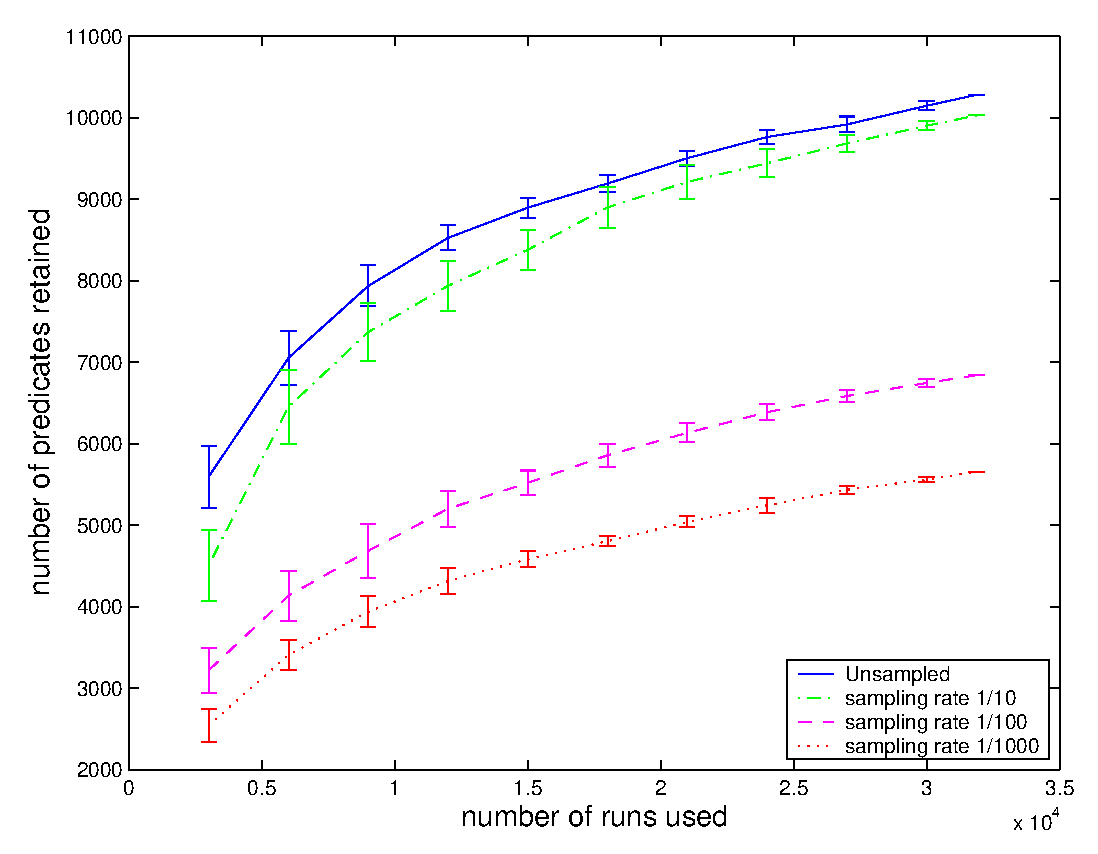
\includegraphics[width=\columnwidth]{predkept3a}\label{fig:predkept-a}}
  \hfill
  \subfigureautorefname[branches and returns only]{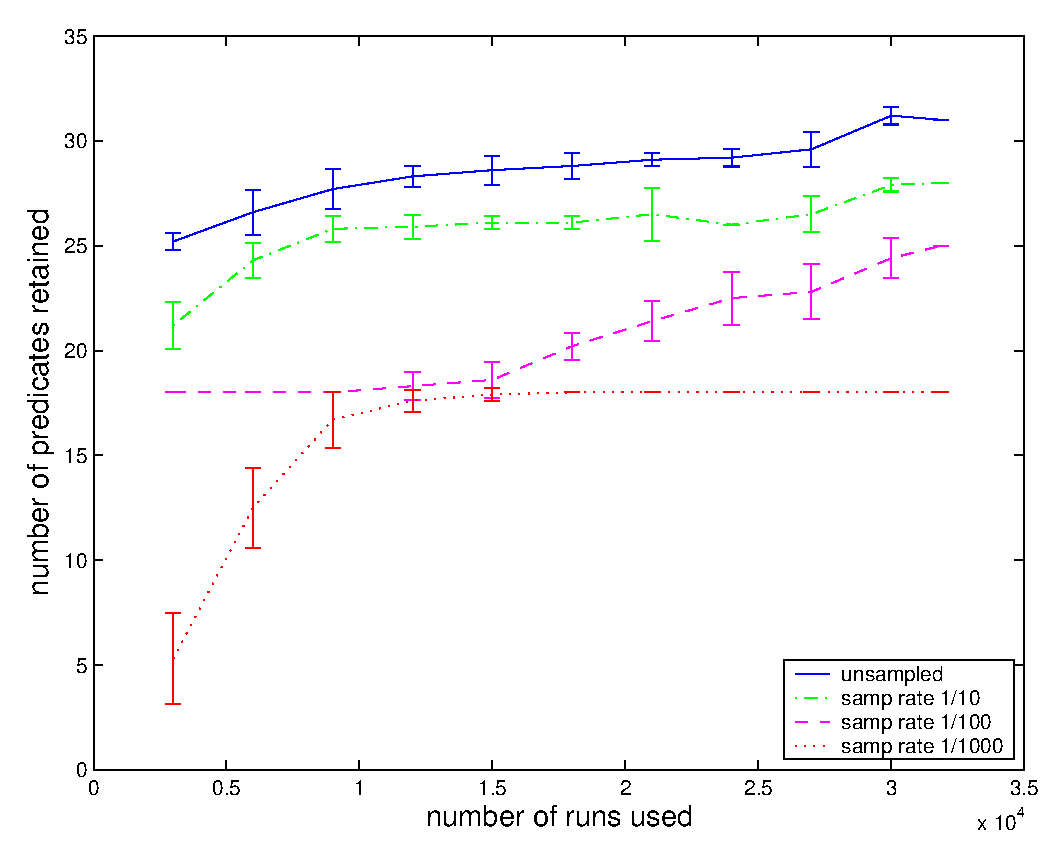
\includegraphics[width=\columnwidth]{predkept3b}\label{fig:predkept-b}}

  \caption{The effect of sampling and data size on the number of
  predicates selected.}\label{fig:predkept}
\end{figure*}

Two trends are apparent from \Autoref{fig:predkept}.  As one would expect,
the number of retained predicates decreases as the sampling rate decreases,
and increases as more trial runs are included.  If we had an unlimited number
of trial runs, the number of retained predicates at all sampling rates should
approach the result with no sampling.  

Note also that increasing 
the number of trial runs always seems to increase the number of retained 
scalar-pairs predicates, whereas the branch and returns predicates run into 
a plateau at lower sampling rates.  Though there may not be much significance 
in this discovery, we conjecture that it is due to the fact that scalar
pairs predicates are much more often observed than the other two kinds of
predicates.  Therefore determining the importance of scalar pairs predicates
takes much fewer sampled trial runs.

%% As is apparent from the graph, there is much larger variation in the
%% number of selected predicates when we use fewer trial runs.
%% %Using $3000$ trials, at the minimum we
%% %retain $7429$ predicates using unsampled data, $7654$ when sampling
%% %rate is $\nicefrac{1}{10}$, $7347$ at $\nicefrac{1}{100}$, and $6750$
%% %at $\nicefrac{1}{1000}$;
%% As we incorporate more examples of successful and failed \moss\ runs,
%% the variances decrease for all sampling rates, but the means behave
%% somewhat differently.  When the data is not sampled, the average
%% number of selected predicates stays around $8100$ for all data sizes.
%% Sampling adds noise to this procedure.  As we observed previously,
%% a moderate sampling rate tends to drive up the $\increase(\ldots)$ scores, and
%% thus enlarges our set of selected predicates (except when we are using
%% very few trial runs).

%% At the relatively high sampling rate of
%% \nicefrac{1}{10}, there are still enough samples taken at most
%% instrumentation sites, and there is a net increase in the number of
%% selected predicates.  Once the sampling rate shrinks to
%% \nicefrac{1}{100} and below, however, the effect of sparse
%% sampling sets in.  Fewer samples are taken overall on fewer predicates,
%% and as a result, fewer predicates have a nonzero $\increase(\ldots)$ score.
%% Incorporating more runs tends to alleviate the situation; at above
%% 10,000 runs, roughly the same number of predicates are retained for
%% the \nicefrac{1}{100} sampled data as the complete data.  The very
%% sparse sampling rate of \nicefrac{1}{1000}, on the other hand,
%% causes much more change in the final result.  A lot more predicates
%% are eliminated when using fewer trials, and a lot more predicates are
%% retained using more trials.

%% Most of the volatility in the results come from the scalar-pair
%% predicates.  \Autoref{fig:predkept-b} shows the same graph for
%% only the branch and return predicates.  Here, across all data sizes,
%% the number of selected predicates remains roughly constant at each
%% sampling rate.  The complete data is still able to select the fewest
%% number of predicates, with \nicefrac{1}{100} sampled data following
%% close behind.  The \nicefrac{1}{1000} sampled data still produces a
%% net increase in the number of selected predicates.

%% LocalWords:  downsampling lang downsampled predelim predkept




\section{Previous and Related Work}
\label{sec:related-work}

In this section we briefly survey related work. There is currently a
great deal of interest in applying static analysis to improve software
quality.  While we firmly believe in the use of static analysis to
find and prevent bugs, our dynamic approach has advantages as well.  A dynamic
analysis can observe actual run-time values, which is often better
than either making a very conservative static assumption about run-time
values for the sake of soundness, or allowing some even very simple bugs to escape
undetected.  Another advantage of dynamic analysis, especially one
that uses actual user executions for its data, is the ability to
assign an accurate importance to each bug.  Additionally, as we have shown,
a dynamic analysis that does not require an explicit specification of
the properties to check can find clues to a very wide range of errors,
including classes of errors not considered in the design of the
analysis.
  
The Daikon project \cite{ernst2001} monitors instrumented applications
to discover likely program invariants.  It collects extensive trace
information at run time and mines traces offline to accept or reject any
of a wide variety of guessed candidate predicates.  The DIDUCE project
\cite{ICSE02*291} tests a more restricted set of predicates within the
client program, and attempts to relate state changes in candidate
predicates to manifestation of bugs.  Both projects assume complete
monitoring, such as within a controlled test environment.  Our goal is
to use lightweight partial monitoring, suitable for either for testing
or deployment to end users.  We never have complete information, and
therefore we must use a more statistical approach.

\termdef{Software tomography} as realized through the GAMMA system
\cite{PASTE'02*2,Orso:2003:LFDIART} shares our goal of low-overhead
distributed monitoring of deployed code.  GAMMA collects code coverage
data to support a variety of code evolution tasks.  Our
instrumentation exposes a broader family of data- and
control-dependent predicates on program behavior and uses randomized
sparse sampling to control overhead.  Our
predicates do, however, give coverage information: the sum of all predicate counters at a site converges to the relative coverage of that site.

Efforts to directly apply statistical modeling principles to debugging
have met with mixed results.  Early work in this area by Burnell and
Horvitz \cite{Burnell:1995:SCM} uses program slicing in conjunction
with Bayesian belief networks to filter and rank the possible causes
for a given bug.  Empirical evaluation shows that the slicing component
alone finds 65\% of bug causes, while the probabilistic model
correctly identifies another 10\%.  This additional payoff may seem
small in light of the effort, measured in multiple
man-years, required to distill experts' often tacit knowledge into a
formal belief network.  However, the approach does illustrate one
strategy for integrating information about program structure into the
statistical modeling process.

In more recent work, Podgurski et al.\ \cite{ICSE`03*465} apply
statistical feature selection, clustering, and multivariate
visualization techniques to the task of classifying software failure
reports.  The intent is to bucket each report into an equivalence
group believed to share the same underlying cause.  Features are
derived offline from fine-grained execution traces without sampling;
this approach reduces the noise level of the data but greatly restricts the
instrumentation schemes that are practical to deploy outside of a
controlled testing environment.  As in our own earlier work, Podgurski
uses logistic regression to select features which are highly
predictive of failure.  
Clustering tends to identify small, tight groups of runs which do
share a single cause but which are not always maximal.  That is, one
cause may be split across several clusters.

In contrast, current
industrial practice uses stack traces to cluster failure reports into
equivalence classes.  Two crash reports showing the same stack trace,
or perhaps only the same top-of-stack function, are presumed to be two
reports of the same failure.  This heuristic works to the extent that a single
cause corresponds to a single point of failure, but our experience
with \moss, \rhythmbox, and \exif suggests that this assumption may not often hold.  In \moss,
we find that only bugs \#2 and \#5 have truly unique ``signature'' stacks: a
crash location which is present if and only if the corresponding bug
was actually triggered.  These bugs are also our most deterministic.
Bugs \#4 and \#6 also have nearly unique stack signatures.
The remaining bugs are much less consistent: each stack signature is
observed after a variety of different bugs, and each triggered bug
causes failure in a variety of different stack states.  \rhythmbox and \exif
bugs caused crashes so long after the bad behavior that the crash stacks
were not useful at all.

Studies that attempt real-world deployment of monitored software must
address a host of practical engineering concerns, from distribution to
installation to user support to data collection and warehousing.
Elbaum and Hardojo \cite{Elbaum:2003:DISATA} have reported on a
limited deployment of instrumented Pine binaries.  Their experiences
have helped to guide our own design of a wide public deployment of
applications with sampled instrumentation, presently underway
\cite{Liblit:2004:PDCBI}.

For some highly available systems, even a single failure must be
avoided.  Once the behaviors that predict imminent failure are known,
automatic corrective measures may be able to prevent the failure from
occurring at all.  The Software Dependability Framework (SDF)
\cite{Gross:2003:PSMUST} uses multivariate state estimation
techniques to model and thereby predict impending system failures.
Instrumentation is assumed to be complete and is typically
domain-specific.

\issue[Alex]{There is a new Ernst paper in FSE and there was another
  one in ICSE\@.  I'm not sure either is really relevant, but if we are
  going to cite him we should show awareness of the more recent work.}

\issue[Alex]{I don't know what Orso has been doing other than that he
  told me they have done a study on whether code coverage in the field
  is similar to code coverage in testing; we should cite that one.
  It's on his home page, I'm pretty sure (Alessandro Orso, I think, at
  Georgia Tech).}

\issue[Mayur]{Add references to Ernst and Orso.  [I think we already
  have enough references to these folks and the related work section
  is already quite long.  Let us give this the least priority.]}

\subsection{Comparison with Logistic Regression}
\label{sec:comparison}

\begin{table}
\caption{Results of logistic regression for \moss}
\label{tab:logregression}
\centering
\small
\begin{tabular}{ll}
  \toprule
  Coefficient & Predicate \\
  \midrule
  0.769379 & \verb|p + passage_index)->last_line < 4| \\
  0.686149 & \verb|(p + passage_index)->first_line < i| \\
  0.675982 & \verb|i > 20| \\
  0.671991 & \verb|i > 26| \\
  0.619479 & \verb|(p + passage_index)->last_line < i| \\
  0.600712 & \verb|i > 23| \\
  0.591044 & \verb|(p + passage_index)->last_line == next| \\
  0.567753 & \verb|i > 22| \\
  0.544829 & \verb|i > 25| \\
  0.536122 & \verb|i > 28| \\
  \bottomrule
\end{tabular}
\end{table}

In earlier work 
we used $\ell_1$-regularized logistic regression
to rank the predicates by their
failure-prediction strength \cite{PLDI`03*141,NIPS2003_AP05}.
Logistic regression uses linearly weighted
combinations of predicates to classify a trial run as successful or
failed.  Regularized logistic regression incorporates a penalty
forcing most coefficients to be set to zero, thereby
selecting only the most important predicates.  The output is a set of
coefficients for predicates giving the best overall prediction.

A weakness of logistic regression for our application is that it seeks
to cover the set of failing runs without regard to the orthogonality
of the selected predicates (i.e., whether they represent distinct
bugs).  This problem can be seen in \autoref{tab:logregression},
which gives the top ten predicates selected by logistic regression
for \moss.  The striking fact is that all selected predicates are
either sub-bug or super-bug predictors.  The predicates beginning {\tt
p + \ldots} are all sub-bug predictors of bug \#1 (see
\autoref{tab:mossdilute}).  The predicates {\tt i > \ldots} are
super-bug predictors: {\tt i} is the length of the command line and
the predicates say program crashes are more likely for long command
lines (recall \autoref{sec:introduction}).

The prevalence of super-bug predictors on the list shows the
difficulty of making use of the penalty term.  Limiting the number of
predicates that can be selected via a penalty has the effect of
encouraging logistic regression to choose super-bug predictors, as
these cover more failing runs at the expense of poorer predictive
power compared to predictors of individual bugs.  On the other hand,
some of the predicates are apparently excellent sub-bug predictors,
and are therefore chosen over others.
%%Relaxing the penalty
%%allows logistic regression to add more predicates to improve its
%%prediction, but the sub-bug predictors apparently are favored.

\section{Conclusions}
\label{sec:conclusions}

We have demonstrated a practical, scalable algorithm for isolating multiple bugs
in complex software systems.  Our experimental results show that we can
detect a wide variety of both anticipated and unanticipated causes of failure
in realistic systems and do so with a relatively modest number of program
executions.

%{\small
\bibliography{cacm1990,gcbib,icse02,icse03,misc,nips16,paste02,pldi03,pods,ramss,refs}
%}
\end{document}

%% LocalWords:  DIDUCE Burnell Horvitz Podgurski Elbaum Hardojo SDF CCured
%% LocalWords:  topcrash cacm icse ramss pldi Podgurski's Kanduri logregression
%% LocalWords:  McMaster Umranov Votta mossdilute gcbib
